%==============================================================================
% Sjabloon poster bachproef
%==============================================================================
% Gebaseerd op document class `a0poster' door Gerlinde Kettl en Matthias Weiser
% Aangepast voor gebruik aan HOGENT door Jens Buysse en Bert Van Vreckem

\documentclass[a0,portrait]{hogent-poster}

% Info over de opleiding
\course{Bachelorproef}
\studyprogramme{toegepaste informatica}
\academicyear{2022-2023}
\institution{Hogeschool Gent, Valentin Vaerwyckweg 1, 9000 Gent}

% Info over de bachelorproef
\title{Het verbinden van een card reader met een webapplicatie.}
\subtitle{Een vergelijkende studie en proof of concept}
\author{Wout De Maeseneer}
\email{wout.demaeseneer@student.hogent.be}
\supervisor{Gertjan Bosteels}
\cosupervisor{Kevin Lommens (Jan De Nul)}

% Indien ingevuld, wordt deze informatie toegevoegd aan het einde van de
% abstract. Zet in commentaar als je dit niet wilt.
\specialisation{Mobile \& Enterprise development}
\keywords{MiFare card; chip card; card reader, Windows Service, SignalR, WebUSB}
%\projectrepo{https://github.com/user/repo}

\begin{document}

\maketitle

\begin{abstract}
Jan De Nul zoekt de beste manier om een kaartlezer te kunnen gebruiken binnen hun webapplicatie. In deze bachelorproef werd dit onderzocht. Twee mogelijke oplossingen werden hiervoor (wanneer mogelijk) uitgewerkt tot een Proof of Concept. Één werkte met WebUSB en de andere met een Windows Service en SignalR. Hier kwam de oplossing met Windows Service en SignalR als enigste werkende oplossing uit.
\end{abstract}

\begin{multicols}{2} % This is how many columns your poster will be broken into, a portrait poster is generally split into 2 columns

\section{Introductie}

Stel dat het gebouw moet geëvacueerd worden, maar er is niet geweten wie er zich allemaal in het gebouw bevindt, toegangspassen zijn daarvoor de oplossing.
Om toegangspassen en maaltijdcheques in te scannen heeft Jan De Nul een webapplicatie nodig die met een card reader deze kaarten rechtstreeks kan inlezen in de browser, hiervoor moet WebUSB worden gebruikt of een driver worden voorzien.
Wat is de beste manier om een card reader te verbinden met een webapplicatie in de browser? 
Er zal een Proof of Concept worden gemaakt die zal worden gebruikt binnen de badges webapplicatie van Jan De Nul. Deze webapplicatie zal onder andere nieuwe kaarten aan het systeem moeten kunnen toevoegen. Er zal dus een MiFare-kaart worden gescand en de tag van de kaart zal via de Proof of Concept op de site verschijnen zodat deze kan worden toegevoegd in het systeem.

\section{Onderzoek}
WebUSB kwam na de literatuurstudie als enige mogelijke oplossing naar boven die al wordt ondersteund door browsers. De tweede mogelijke oplossing kwam er na een interview met Anton D'hondt. Hij had het idee om met behulp van een Windows Service en SignalR de kaart data door te sturen naar de webapplicatie. Vervolgens werden de mogelijke oplossingen (wanneer mogelijk) uitgewerkt tot een Proof of Concept. Tenslotte werd er nog gecheckt of de tag binnen de seconde op de webapplicatie verschijnt.

%\section{Sectie met figuur}

%De {\LaTeX} figure-omgeving bepaalt zelf waar een afbeelding komt en dat is meestal niet op de plek in de tekst waar de figure-omgeving gedefinieerd wordt. Als je wilt forceren dat afbeeldingen toch in de flow van de tekst blijven, dan kan je dat zoals hieronder:

\begin{center}
  \captionsetup{type=figure}
  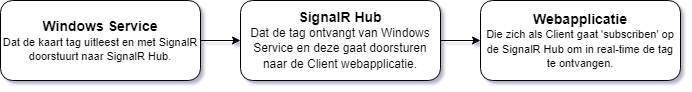
\includegraphics[width=1.0\linewidth]{BP_voorbeeld_schema.drawio}
  \captionof{figure}{Schema dat toont hoe het idee met Windows Service en SignalR in elkaar zit.}
\end{center}

%Let er wel op dat dit tot problemen met bladschikking kan leiden.

\section{Conclusies}

Uit dit onderzoek kan geconcludeerd worden dat data van een smartcard met een card reader naar een webapplicatie versturen niet iets voor de hand liggend is. Er is gebleken dat WebUSB geen oplossing is. Dit komt omdat de card reader niet kan worden gebruikt met WebUSB wegens security issues, omdat er mogelijks belangrijke data aan te pas komt bij het uitlezen van de smartcard. 
Er werd ook een interview afgelegd met Anton D'hondt waarin hij zijn idee tot een mogelijke oplossing uitlegde. Zijn idee werd vervolgens uitgewerkt tot een Proof of Concept. En uit deze Proof of Concept kan geconcludeerd worden dat het een oplossing is omdat het werkt en het onder een seconde de tag op de webapplicatie laat verschijnen. 
Het antwoord op de onderzoeksvraag biedt een meerwaarde voor Jan De Nul. Om de webapplicatie van JDN te kunnen gebruiken moest het mogelijk zijn om met hun ACR122U card reader de data van een kaart uit te lezen naar de webapplicatie. De Proof of Concept die ik voor deze bachelorproef heb uitgewerkt zal dus worden gebruikt in die webapplicatie. Ik denk wel dat de Proof of Concept met SignalR en Windows Services duidelijk en goed in elkaar zit en het een volwaardige oplossing is tot de onderzoeksvraag.

\section{Toekomstig onderzoek}

Bijkomend onderzoek is nodig om de Proof of Concept te laten werken met andere soorten smartcards. In de toekomst is Jan De Nul namelijk van plan om MiFare DESFire kaarten te gaan gebruiken. En de het zal ook de bedoeling zijn om maaltijdcheque kaarten te gebruiken. De maaltijdcheque kaarten zijn gelijkaardig aan bankkaarten, ze bevatten een chip en kunnen ook draadloos worden gebruikt. Deze kaarten werken dus met iets andere technologie waardoor er nog toekomstig onderzoek zal moeten worden gedaan om de Proof of Concept aan te passen zodat deze werkt met deze technologie.

\end{multicols}
\end{document}